%%%%%%%%%%%%%%%%%%%%%%%%%%%%%%%%%%%%%%%%%%%%%%%%%%%%%%%%%%%%%%%%%%%%%%%%
%                                                                      %
%     File: Thesis_Background.tex                                      %
%     Tex Master: Thesis.tex                                           %
%                                                                      %
%     Author: João C. Godinho                                          %
%     Last modified : Apr 2018                                         %
%                                                                      %
%%%%%%%%%%%%%%%%%%%%%%%%%%%%%%%%%%%%%%%%%%%%%%%%%%%%%%%%%%%%%%%%%%%%%%%%

\chapter{Related Work}
\label{chapter:related_work}

The following chapter will go over prior work that closely relates to the topic of our research and areas of contribution.
We approach the definition of malware and how it can be hard to detect and label by providing some background on the subject.
We then proceed to elucidate on different malware detection techniques, from simple methods to more complex approaches, focusing on a specific malware analysis technique that provided the basis for our work.

We advance to the general topic of \gls{ml}, after which we describe related work that studies the use of \gls{ml} in malware detection.
Lastly, we reference prior work that not only tackles our same goal, but also takes into account the impact of \textit{laboratory} \textit{vs.} \textit{real world} scenarios, as well as the notion of temporal based detection, or concept drift.

%%%%%%%%%%%%%%%%%%%%%%%%%%%%%%%%%%%%%%%%%%%%%%%%%%%%%%%%%%%%%%%%%%%%%%%%
\section{Background}
\label{section:background}

The term malware was first used by Yisrael Radai in 1990~\cite{elisan:malware}, before then malicious software was referred to as computer viruses, a notion which was first formalized by Cohen in 1983~\cite{cohen:virus}.
Given term computer virus predates the term malware, it is not uncommon to see both terms used interchangeably.
% For the purpose of this work the term malware is adopted, for reasons explained in the following paragraphs.

To the exponential growth of malware~\cite{av-test:report}, the ability to distinguish between malware samples is crucial.
In the biological world, different types of infections reckon distinctive disinfections, the same applies to the digital world.
The infection method, behavior and subsequently purpose of malware samples vary, hence being able to make a distinction facilitates prevention and disinfection by anti-virus solutions.

There exists no ground truth when it comes to distinguishing malware, leading to subtle differences on the classification and naming of the same malware instance by different parties.
To facilitate the reader's understanding of the topic, the current work will focus on defining malware types based on their propagation and purpose.

With respect to the propagation method, malware can be split into three classes~\cite{kolter:learning}:

\paragraph{Virus.}%\footnote{This work uses virus as a subset of malicious code, hence the choice of using the term malware over virus.}
This type of malware inherits its name from resembling to biological viruses.
A virus is usually composed by two main subroutines.
The first subroutine is responsible for infecting other programs by attaching the virus code, while the second subroutine is the actual malware payload that contains the malware purpose (\ie\ virus payload)~\cite{chen:evolution}.
Viruses are attached to programs and propagate when an infected program is run, either consciously (\eg\ clicking on executables) or unconsciously (\eg\ auto-run features), hence depending on other programs (as hosts) and user interaction.
For viruses to infect new systems, an infected file must be carried between them by a user (\eg\ USB pen, email attachment), reinforcing the user's role in this propagation method.

\paragraph{Worm.} The increasing number of network connected devices facilitates the application of worms to propagate malware.
A worm shares the self-replicating ability of viruses, but discards user interaction and the need for a host.
This is possible by making a worm an independent program that exploits networks to find vulnerable systems to infect with a copy of themselves~\cite{chen:evolution}.
Similarly to viruses, worms can contain additional payload to perform malicious actions on infected systems (\eg\ Blaster worm exploited a vulnerability in RPC for propagation while its payload flooded a Microsoft domain\footnote{W32/Blaster worm, CERT, August 11, 2003 [http://www.cert.org/historical/advisories/CA-2003-20.cfm]}).

\paragraph{Trojan.} While viruses and worms focus on self-propagation, trojans focus on deceiving users into executing them, disregarding propagation.
Trojans try to appeal users with some useful functionality as to allure into running the program~\cite{szor:art}.
By hoaxing users into running them, trojans bypass the need for a host (in the virus case) or an exploit (in the worm case) to perform malicious actions.

\medskip

These three classes are not exclusive and can be used in conjunction to facilitate propagation (\eg\ a virus that relies on a trojan to start propagating).
Given the inexistent standards for malware naming, some literature~\cite{szor:art} define worms as a subset of viruses, as some worms start by attaching to files.
With the general infection methods layered out, the following will succinctly describe the general naming when referring to the malware purpose (\ie\ its payload).

Given the high numbers of malware multiple purposes imply multiple names, as such the following lists some of the most commonly heard names and definitions as given by McAfee~\cite{mcafee:glossary}:

\begin{itemize}
	\item \textit{Adware}: Program that automatically displays advertisement to the user. Most do not cause direct harm.
	\item \textit{Backdoor}: Installs or takes advantage of an unknown entry point to a user's system, allowing remote control of a system.
	\item \textit{Bot}: Short for \say{robot}; A program that receives commands from a cybercriminal and executes them blindly, due to this characteristic, compromised computers are called zombies.
	\item \textit{Dropper}: Program that facilitates the introduction of other malware instances into a system.
	\item \textit{Keylogger}: Program that monitors a user's input (\eg\ keyboard strokes) to steal private information.
	\item \textit{Password Stealer (PWS)}: Program that specifically targets a user's personal information, like usernames and passwords.
	\item \textit{Ransomware}: Program that restricts access to a system/files (usually by encryption) and demands a ransom to allow a user his access.
	\item \textit{Remote Administration Tool - RAT}: Program designed to give an administrator remote control of a system. Similar to \textit{Backdoor} and \textit{Bot}, but usually has higher privileges on infected systems.
	\item \textit{Rootkit}: Program designed to hide the existence of other (malicious) programs, hindering detection of malicious applications.
	\item \textit{Scareware}: Program that fakes the existence of malware and tricks the user into paying for disinfection or into downloading real malware.
	\item \textit{Spyware}: Program that spies on a user's activity through multiple vectors (\eg\ taking prints of a user's desktop/webcam).
\end{itemize}

The ability to name a malware given its propagation method and purpose facilitates detection and disinfection, but given the high quantities of malware, being able to particularly discriminate an instance is helpful.
To that purpose, attempts have been made to create naming conventions for malware.

One of the first attempts was made in 1991, by the \gls{caro}~\cite{caro:naming}.
This attempt was aimed at viruses only and focused on discriminating and relating virus samples.
The convention defines an hierarchical naming with three levels.
The base of the hierarchy is the family name, where structurally similar virus should be grouped.
To further distinguish instances, a group name and major variant name is applied.
To differentiate versions of the same instance and provide additional information about a sample, minor variant name and modifier fields are to be used.
In sum, a virus name should look as following:

\begin{center}\texttt{family.group.major.minor:modifier}\end{center}

To enable differentiation from other types of malware, an improvement to \gls{caro}'s naming was proposed in 1999 by Geral Scheidl~\cite{scheidl:naming}.
Scheidl's proposal included a prefix that consisted of the platform targeted by the malware and a type (\ie\ previously defined classes and names), rendering a more in-depth name:

\begin{center}\texttt{platform.type/family.group.major.minor:modifier}\end{center}

In the Virus Bulletin magazine of January 2002~\cite{virus_bulletin} the naming problem is again addressed, referencing that only a small number of vendors apply \gls{caro}'s names and that the lack of cooperation between anti-virus vendors lead to multiple aliases for malware names.
Again a naming convention is proposed with focus on detail by using three levels of information: malware name, classification and full text description.

Given that no naming convention is widely adopted, anti-virus vendors make use of their own naming that although similar, vary slightly.
This variation raises the redundancy for instances of the same malware as shown by an article published by Symantec in 2002\footnote{A Virus by Any Other Name: Virus Naming Pratices, Costin Riau, June 2, 2002 [https://www.symantec.com/connect/articles/virus-any-other-name-virus-naming-practices]}, stating that the same malware instance has an average of four different names.

The naming problem, although not directly related to the current work, must be taken into consideration as to not influence the classification results.

%%%%%%%%%%%%%%%%%%%%%%%%%%%%%%%%%%%%%%%%%%%%%%%%%%%%%%%%%%%%%%%%%%%%%%%%
\section{Malware Detection}
\label{section:mal_detec}

This section will provide a deeper description of detection methods, from the simplest techniques to more complex ones. The following is based on the work by Peter Szor, \textit{The Art of Computer Virus Research and Defense}~\cite{szor:art}, which although not recent, provides a solid background on detection methods.

To detect malware instances, anti-virus applications are used.
These can also be called scanners, as early detection methods simply scanned for byte sequences to detect malware.
Before going into details on the different detection techniques, it is worth mentioning that scanners can be used as \textit{on-demand} or \textit{on-access} scanners.
On-demand anti-virus are executed only at the user's request.
On-access anti-virus are memory-resident, meaning they load as an application and intercept actions related to file and disk access.
This makes it so that when files are opened, created or closed, the anti-virus scans the changed object.

%%%%%%%%%%%%%%%%%%%%%%%%%%%%%%%%%%%%%%%%%%%%%%%%%%%%%%%%%%%%%%%%%%%%%%%%
\subsubsection{First-Generation Scanners}
\label{subsection:first_gen_scanners}

These type of scanners work at a fairly simple level and focus searching for known byte sequences (\ie\ known to be malware sequences).
The applied principles include:

\paragraph{String Scanning.} A sequence of bytes that is common in a malicious program but not in a regular program is matched against a suspicious file. 

\paragraph{Wildcards.} This method is similar to string scanning, but instead of searching for a fixed sequence of bytes, a more flexible matching is made, allowing to skip bytes or byte ranges.
The method can also include the use of regular expressions for matching.

\paragraph{Mismatches.} Also similar to string scanning, yet there can be $N$ number of bytes in the string that can take any value and in any position (\eg\ the string \say{\texttt{01 02}} with mistmatch of 1 matches \say{\texttt{01 AA}} and \say{\texttt{AA 02}}).

\paragraph{Generic Detection.} This method typically applies both wildcards and mismatches to create generic strings that can scan for several variants of a family of malware, hence being more robust to subtle changes in malware.

\medskip

These principles can be assigned to the signature-based type of methods, as they depend on searching some previously defined byte sequence to be effective.
Their effectiveness depends on an updated knowledge base with the strings to be matched.

Alongside these basic principles, the following can be used in conjunction to improve the scanning speed and reliability:

\paragraph{Hashing.} This term is not a method by itself, but techniques that speed up searching algorithms, enhancing previous methods.
It takes advantage of the hash table data structure to match malware signatures.

\paragraph{Bookmarks.} This method is both used to provide more accurate detections and disinfections. Bookmarks provide specific locations for where strings are to be searched (\ie\ offsets).

\paragraph{Top-and-Tail Scanning.} Like hashing, this principle is used to speed up detection by scanning the start and end of a file, instead of the entire file.
The technique is mainly effective when dealing with viruses that prefix or append data to files.

\paragraph{Entry-Point and Fixed-Point Scanning.} This technique also improves the speed of anti-virus scanners.
By taking advantage of the structure of binary objects this method can start scanning at the entry-point of an object, or alternatively use the entry-point plus some fixed size as a fixed-point from where to start scanning.

\paragraph{Hyperfast Disk Access.} This last technique also provides a speed improvement.
It does so by bypassing operating system level \gls{api} to read the disk directly with the \gls{bios}.
In addition to improve the scanners performance, this principle is also useful as an anti-stealth technique, given it works below the filesystem layer.
It is worth noting that this technique is hard to implement nowadays due to the high variety of file systems and disk controllers.

%%%%%%%%%%%%%%%%%%%%%%%%%%%%%%%%%%%%%%%%%%%%%%%%%%%%%%%%%%%%%%%%%%%%%%%%
\subsubsection{Second-Generation Scanners}
\label{subsection:second_gen_scanners}

These methods improve on the previous generation by doing an analysis at a higher level of abstraction.
Where first-generation scanners would match sequences of bytes, second-generation scanners also look at the bytes representation.
The applied principles include:

\paragraph{Smart Scanning.} This method takes the assembly representation of the bytes into account and instructions that have no effect (\eg\ \texttt{NOP}) can be skipped.
The resulting signature is smaller and more easily detects mutations.
The same principle can be applied to textual malware (\eg\ scripts), where extra white spaces have no effect.

\paragraph{Skeleton Detection.} This method is specifically useful in detecting textual malware (\eg\ macros) families.
By parsing the macro statements line by line, the scanner can drop nonessential statements.
The result can be seen as a skeleton of the full macro that contains only the relevant code that appears in malware.

\paragraph{Nearly Exact Identification.} This method provides a more accurate way to detect malware.
First-generation scanners base detection mainly on a byte sequence, whereas nearly exact identification makes use of double-string detection.
The principle comes from using two strings to match a given malware, if only one of those strings match, then it is likely to be a variant of a known malware.
This is specifically useful to identify same family malware.
Another nearly exact identification method applies a checksum to a range from the malware body, this has the added benefit of better accuracy without overloading the anti-virus database.

\paragraph{Exact Identification.} This method enhances the previous method by adding the ability to differentiate malware variants.
It does so by using as many checksum ranges as needed to identify variants of the same malware, improving the accuracy and facilitating disinfection.

\medskip

Like in the previous generation, these methods fit into signature-based, hence still being highly dependent on an updated knowledge base.

%%%%%%%%%%%%%%%%%%%%%%%%%%%%%%%%%%%%%%%%%%%%%%%%%%%%%%%%%%%%%%%%%%%%%%%%
\subsubsection{Algorithmic Scanning Methods}
\label{subsection:algorithmic_scanning}

These methods are not so focused on direct matching of signatures, but on the routines implemented in the scanner that allow the detection of malware.
Early implementations of algorithmic scanning were hard-coded in the anti-virus, but with different types and families emerging, the hard-coded algorithms could easily become obsolete.
To overcome this, vendors would introduce more specific routines for malicious programs when updating the anti-virus.

Examples of these methods are filtering, where signatures are only applied if an object meets a particular filter; static decryptor, which detects encrypted malware; and X-ray, which tries to decrypt malware that use simple encryption methods (e.g. \say{\texttt{XOR}} with constant key).

Algorithmic scanning methods are more related to heuristic-based methods, since the focus is developing rules to facilitate malware detection and removal.
These methods also allow for vendors to push new detection algorithms to clients without having to update the entire anti-virus.

%%%%%%%%%%%%%%%%%%%%%%%%%%%%%%%%%%%%%%%%%%%%%%%%%%%%%%%%%%%%%%%%%%%%%%%%
\subsubsection{Code Emulation}
\label{subsection:code_emulation}

This detection technique uses dynamic analysis (\ie\ analysis during runtime) to detect malware by simulating code execution.
A virtual machine is used to simulate the system's components, thus the malicious files are encapsulated and no code is executed by the real processor.

Code emulation can be faster than using algorithmic scanning methods when dealing with encrypted/obfuscated malware, as the code can be emulated and the decrypted/deobfuscated code is much easier to obtain.
The downside to emulation comes from a time perspective, as more resources are needed to emulate code.

%%%%%%%%%%%%%%%%%%%%%%%%%%%%%%%%%%%%%%%%%%%%%%%%%%%%%%%%%%%%%%%%%%%%%%%%
\subsubsection{Heuristic Analysis}
\label{subsection:heuristic_analysis}

This detection technique takes into account several characteristics of malicious software, both static and dynamic.
Examples of such characteristics are code execution starting in uncommon sections, suspicious code redirection or incorrect size of code in header.

Using the previously described methods, heuristic analysis can take into account different characteristics that are present or absent to assert if a file is deemed malicious or not.

The upside of this technique is that it allows for never seen malware to be correctly flagged, but brings the downside of a higher amount of false positives.

%%%%%%%%%%%%%%%%%%%%%%%%%%%%%%%%%%%%%%%%%%%%%%%%%%%%%%%%%%%%%%%%%%%%%%%%
\subsubsection{Sand-Boxing}
\label{subsection:sand_boxing}

This detection technique builds on the already mentioned code emulation, but with a higher level of complexity.
With sand-boxing the whole system is emulated (\ie\ virtualized) and suspicious or malicious programs have access to a copy of the real resources, effectively limiting the effects of the program and consequently protecting the system.

This technique allows to extract dynamic information without compromising the real system, which can then be used to detect if a suspicious program is malware, by applying the aforementioned techniques, and to help analyze new types of malware.
This technique demands more resources then previous ones and may not be ideal to use inside an anti-virus application.

Other downsides of sand-boxing come as compatibility issues, the possibility of malware detecting virtualization, which can hinder analysis, or even if the virtualization software is vulnerable and malicious code can escape the sandbox into the host machine.

\medskip

Detecting malware is not as simple as applying one of the mentioned techniques, different methods work best in different scenarios, hence anti-virus need to balance the usage of these techniques to keep systems protected.

%%%%%%%%%%%%%%%%%%%%%%%%%%%%%%%%%%%%%%%%%%%%%%%%%%%%%%%%%%%%%%%%%%%%%%%%
% TODO mais umas linhas sobre estatico e dinamico
\section{Cuckoo Sandbox and Malwr}
\label{section:cuckoo}

Building on the last described method of sand-boxing, this section will describe a specific implementation of sand-boxing, namely Cuckoo.
Cuckoo Sandbox is a malware analysis system created by Claudio Guarnieri~\cite{tool:cuckoo}.

When analyzing a malware sample, an analyst will have to create his own virtual environment, transfer the sample into that environment and manually interact with the sample to see how it behaves and what it does.
Cuckoo facilitates analysis by automating this process.

The Cuckoo system will take the sample to analyze and run it inside a predefined virtual environment (\eg\ Windows XP).
The system is then capable of simulating user interaction, take screenshots of the environment, extract static and dynamic information about a sample, monitor network traffic and perform memory analysis.
The time spent doing the analysis can be configured by the user.
Upon finishing the analysis the system provides reports about the sample. The reports' information can be divided into 5 sections:
\begin{itemize}
	\item \textbf{Quick Overview} which includes information like: file type and details; analysis duration; signatures (\ie\ predefined patterns Cuckoo deems suspicious); screenshots during runtime; hosts and domains contacted; files, mutexes and registries used.
	\item \textbf{Static Analysis} which includes information like: file version information; file sections; resources (\eg\ icons); statically imported libraries and their functions; output of the \texttt{strings}\footnote{Linux binary that outputs the strings of printable characters in files.} command on the file; VirusTotal~\cite{tool:virustotal} classification report.
	\item \textbf{Behavioral Analysis} which includes information like: spawned processes; \gls{api} call order for each process.
	\item \textbf{Network Analysis} which includes information like: domains and their resolved IPs; HTTP requests; IRC traffic; SMTP traffic.
	\item \textbf{Dropped Files} which includes information about files created by the sample: their size, name and hash.
\end{itemize}

Some of the defined sections are not always available.
Their availability depends both on a successful analysis by Cuckoo, as well as the type of submitted file.
For example, only binary executables (\eg\ \gls{dll}, \gls{pe}) provide static analysis information.
Using the defined sections provided by Cuckoo's reports, one can obtain static and dynamic features from the samples.

The creator of Cuckoo and one of its developers, Alessandro Tanasi, also created a free malware analysis service, Malwr~\cite{tool:malwr}.
This service implements the Cuckoo system and allows users to upload their own files, which are then run with Cuckoo.
The service is presented as a web application that takes in samples and returns a report with Cuckoo's results.
An example of the behavioral analysis (\ie\ created process and \gls{api} calls) can be seen in Figure \ref{fig:malwr_sample}.

\begin{figure}[!htb]
	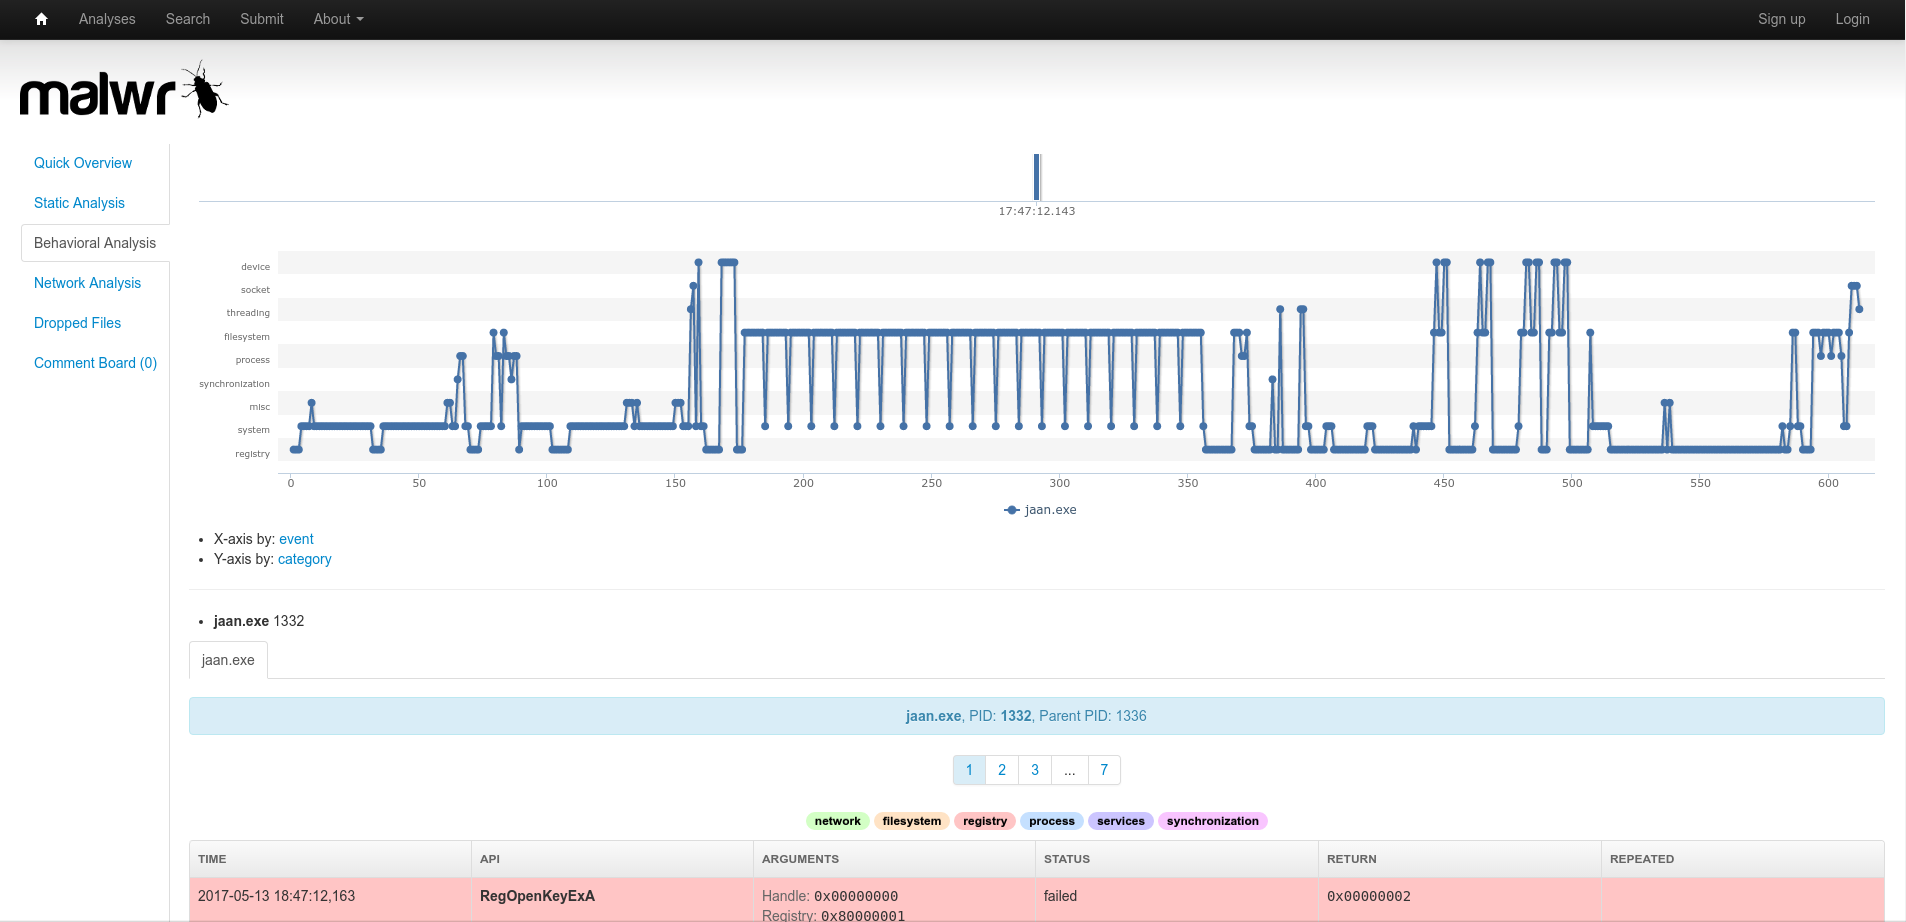
\includegraphics[width=\columnwidth]{Figures/malwr_sample.png}
	\caption{Example of a behavioral report from Malwr.}
	\label{fig:malwr_sample}
\end{figure}

Unfortunately at the time of writing, Malwr is under maintenance hence the provided image will be outdated once the new version is live.

For the purpose of detecting malware via \gls{ml}, the reports provided in Malwr supply various information that can be used for the current work.
The whole website content is provided under \gls{cc} CC-BY-NC-SA 3.0\cite{cc-by-nc-sa} license, allowing use of the data for this work's purpose, as long as credits are maintained.

%%%%%%%%%%%%%%%%%%%%%%%%%%%%%%%%%%%%%%%%%%%%%%%%%%%%%%%%%%%%%%%%%%%%%%%%
\section{Machine Learning}
\label{section:ml}

Even before the modern concept of computer proposed by Alan Turing, mankind has always searched for ways to either automate or facilitate more complex tasks.
With the technological advances that provide higher computation power, computer science fields like \gls{ai} have greatly improved in recent years.

One of the \gls{ai} fields that has benefit from the technological advances is \gls{ml}.
The current subsection will provide a more detailed description of \gls{ml} and its use for the current work.

\gls{ml} is a subset of \gls{ai} in which algorithms are applied to learn and make predictions on data, or more formally defined by Tom Mitchell~\cite{mitchell:ml}:
\begin{center}
\say{\emph{A computer program is said to learn from experience $E$ with respect to some class of tasks $T$ and performance measure $P$, if its performance at tasks in $T$, as measured by $P$, improves with experience $E$.}}
\end{center}

A noteworthy nuance about the given definition, and the \gls{ml} field in general, is that these algorithms are not designed to deal with specific problems.
Meaning that as long as a learning problem is well defined through $T$, $P$ and $E$, an algorithm based on these three features is able to learn, but not necessarily solve any problem.
This creates a contrast to \gls{ai} fields, where algorithms are built for specific tasks.

After defining a learning problem, to obtain a useful outcome (\ie\ model) one or more learning algorithms are applied.
Learning algorithms fall within one of the following classes: \textit{supervised learning}; \textit{unsupervised learning}; \textit{semi-supervised learning} or \textit{reinforcement learning}.

Each of the categories is defined on how the problem is learned . A more detailed description, as seen in \cite{norvig:ai} is as follows:

\paragraph{Supervised Learning.} In this category the program is given a corpus (\ie\ experience) with input-output pairs and it must learn how to map a never seen input into the correct output.
Within supervised learning, a learning problem can be further classified into a classification problem, if the output is a set of finite values (\eg\ is it going to rain tomorrow?), or into a regression problem, if the output is continuous (\eg\ how likely is it to rain tomorrow?).

\paragraph{Unsupervised Learning.} In this category the program is given a corpus and it must learn patterns from the input, hence no correct or wrong output is expected, only how different input relates.
The most common task in unsupervised learning is clustering, where input is grouped based on similar characteristics.

\paragraph{Semi-supervised Learning.} This category is a combination of the previous ones and exists because sometimes the learning problem is based on a dataset that combines both labeled and unlabeled inputs or on a dataset that contains noisy data. 
The combination of supervised and unsupervised learning provides a better overall result in such scenarios.

\paragraph{Reinforcement Learning.} In this category the program is given a problem through a set of states and a set of actions it can perform.
At any given state the program performs an action which results in a reward or punishment.
The cumulative reinforcement at each state teaches the program the best and worse actions for each state.

\medskip

The current work will fit into the supervised learning category, with the purpose of creating a model to assert whether a given sample is malware or not.
This problem can be seen as whether a pure classification problem, with a binary output, or as a regression problem, with the likelihood of a sample being malware.

\medskip

When designing a learning system, multiple choices must be taken into consideration.
A brief description of what should be taken into account is given as seen in~\cite{mitchell:ml}:

\begin{itemize}
	\item \textbf{Training experience} is the first choice, as it can have a significant impact on the success or failure of the learner.
	The feedback provided by the experience can be direct or indirect, affecting the end result of the system.
	Another important aspect is how the experience represents the distribution over which the performance is measured, meaning how well the experience represents the environment where the system is to be used.
	Being what is going to be fed to the learner (\ie\ features), it must be well thought out and understood.
	\item \textbf{Target function} is the next choice, representing what is to be learned.
	The function takes as input the set of features that represent the problem and (ideally) outputs a solution to the task.
	\item \textbf{Target function representation} is the remaining choice, this is where a learning model is applied to learn the given task.
	The choice is of great importance, given it will influence how well the system performs under evaluation.
\end{itemize}

Given the nature of the purposed work as a classification problem, many models can be applied as a representation for the target function.
The following describe some models taken into consideration during implementation.

\paragraph{Decision Tree Learning.~\cite{mitchell:ml}} These methods are used to approximate discrete-valued target functions, where the learned function is represented as a decision tree.
The decision tree is built based on how much information each attribute gives (\ie\ information gain).
These are best suited for problems where instances are represented by attribute-value pairs of discrete values and problems where data may contain errors.
The shortcomings with decision tree methods include how deep to grow the decision tree, how to handle continuous attributes and handling attributes with different weights.

\paragraph{\gls{ann}.~\cite{mitchell:ml}} These methods can be used for real-valued, discrete-valued and vector-valued target functions.
\gls{ann}'s are inspired in part by neurons in the biological world, hence being represented as directed graphs.
\gls{ann}'s can be applied to the same type of problems as decision trees, but these can also handle instances represented by many attribute-value pairs.
\gls{ann}'s have the downsides of being time consuming to train and to easily overfit the training data (\ie\ training data is learned well, but fail to generalize to new data).

\paragraph{Bayesian Learning.~\cite{mitchell:ml}} These methods use a probabilistic approach to inference.
The reasoning is that the optimal decision can be related to some probabilistic distribution of the data.
Bayesian learning proves to be effective for text classification tasks and also provides useful insight on other learning algorithms that do not deal with probabilities.
The shortcomings can be related to the need of requiring initial knowledge, as well as computational cost to achieve the best hypothesis, which grows with the number of hypothesis.

\medskip

Even though the field of \gls{ml} is broad, the main focus is always the ability to generalize a given task.
For every learning task multiple models can be applied, which complicates the task of choosing a model.

Although being able to try different models and how they compare to each other benefits the end result, this work focused solely on a single model, reasoned in Section \ref{section:model_selection_evaluation}.
Doing so enabled to us to spend more time understanding the impacts of \textit{ground-truth} and temporal consistency.

%%%%%%%%%%%%%%%%%%%%%%%%%%%%%%%%%%%%%%%%%%%%%%%%%%%%%%%%%%%%%%%%%%%%%%%%
\section{Machine Learning in Malware Detection}
\label{section:ml_md}

The previous Sections gave a general understanding on how anti-virus software detects malware and how the \gls{ml} field can be applied to learn tasks without having to define specific algorithms.
This section will describe research that aggregates both malware detection and machine learning.
Authors make use of specific \gls{ml} classifiers like Naive Bayes (NB), \gls{lr} and \gls{svm} to design systems that learn to detect malware.

The main focus is to note the choices made by the authors relative to the datasets, classifiers and their evaluation, all of which were taken into consideration in the current work.

\subsection{Best Practices for \gls{ml} in Malware Detection}

Before analyzing the work done with \gls{ml} in malware detection, it is worth noting how such work is to be conducted.

Rossow et al.~\cite{rossow:practices} present some guidelines for designing malware experiments.
Their work surveys 36 academic publications from 2006 to 2011 that rely on malware execution.
The authors note frequent shortcomings in the surveyed publications regarding assumptions on the use of execution-driven datasets, absence of security precautions taken during experiments and insufficient description of the experimental setup.
The provided guidelines are split into four groups: correct datasets, transparency, realism and safety.

Regarding correct datasets, the publication guidelines include whether goodware samples are to be present in datasets, how the dataset is balanced over malware families and if training and evaluation datasets should have different families.
The authors note that at least nine distinct papers suffer from significant problems relating to the correctness criteria.

With regards to transparency, the given guidelines include the interpretation of false positives, false negatives and true positives, family names of employed malware samples and how they were named.
In the surveyed papers, it is noted that the majority do not interpret the numeric results and a fifth do not name the malware families contained in the datasets.

Regarding realism, the paper introduces guidelines which include relevance and variety of malware families and real-world evaluations.
The authors note that only a minority of papers include real-world evaluations and very few offer significant sample sizes, making it difficult to judge practical use of the methodology.

With regards to safety, the given guidelines focus on containment policies when analyzing malware samples.
The authors note that most papers did not deploy or adequately describe containment.

As mentioned in Section \ref{section:cuckoo}, the current work makes use of the reports in Malwr, hence some the guidelines provided in the aforementioned research do not apply, specifically the safety guidelines.
As for the other guidelines, they were taken into consideration when designing the presented learning system.

\medskip 

On the same note of guidelines, Shabtai et al.~\cite{shabtai:survey} provide a survey directed at the application of machine learning classifiers to detect malware from static features.
Their work concerns the design and evaluation of such systems.
The process is divided into two phases: training and testing.

The training phase includes the creation of a feature vector to represent each file and posterior processing of such vectors to generate a classifier.
The testing phase measures the performance of the classifier by employing classical measures like \gls{tpr} (\ie\ detection rate), and \gls{fpr}.

The authors outline that the work in designing learning systems include how the samples are to be represented (\eg\ byte n-grams, portable executable features, strings), methods to select features (\eg\ gain ratio, document frequency) and finally the classification algorithm (\eg\ \gls{ann}, \gls{svm}).

It is noted by the authors that the use of multiple classifiers with different weights (ensembles) is beneficial to the classification task, as different classifiers work better on different features.

Some problems addressed that are of importance for the presented work include the imbalance problem and chronological evaluation.
Having a balanced dataset of malware and goodware might not accurately represent the real world.
For chronological evaluation the question if whether the usage of old samples for training can aid or hinder the classification of new samples.

\subsection{Malware Detection using Static and Dynamic Features}

When it comes to malware detection from static features, Schultz et al.~\cite{schultz:data_mining} present a data-mining framework to detect new, unseen malicious executables.
Their work uses a dataset of 4,266 programs, with 3,625 malicious binaries and 1,001 clean programs, labeled by a commercial anti-virus.
The features include \gls{dll}'s used by the binary, list of \gls{dll} function calls, number of different function calls within each \gls{dll}, strings from the binary and byte sequences.

They apply three different models (RIPPER, Naive Bayes and Multi-Naive Bayes) to different features, achieving a detection rate between 52\% and 98\% and a false positive rate between 5\% and 9\%.
It is worth noting how the application of different models to different features provide very distinct detection rates.
Also worth noting is the size and imbalance of the dataset, where only 23\% of samples are benign in a total universe of 4,266 samples.

The authors describe the malware samples were obtained from various FTP sites and that 5\% were trojans, while the remaining 95\% consisted of viruses, with no remarks are made regarding the involved families.
The majority of benign samples were gathered from a fresh installation of Windows 98, which may not represent the average benign sample.

\medskip

Another application of \gls{ml} to malware detection from static features is done by Nissim et al.~\cite{nissim:al_pdf}.
The authors apply active learning (semi-supervised learning that takes user input) to the detection of malicious PDF files based on static features.
They use a dataset of 6,774 PDF files, including 1,629 malicious and 5,145 benign files, where the benign files were mark as such by Kaspersky anti-virus software.

Their framework works by filtering out all known benign and malicious PDF's and passing the remaining files to a \gls{svm} model, which linearly separates files based on an initial training set of malicious and benign files.
The ones deemed informative are flagged for manual inspecting and used in future iterations of the \gls{svm} model training.
The core idea in this work is to focus on detecting new and unseen instances of malware files with the help of human interaction.

The authors only apply an \gls{svm} model and justify its use due to previous work that provided good results in malware detection, the fact that it is hard for attackers to understand how the model separates files, that it is efficient when combined with active learning and the ability to handle large number of features.

They evaluate their framework by creating 10 subsets of 620 files, with the remaining 574 files used as initial training for the \gls{svm} model.
For each subset the \gls{svm} is trained and choses the most informative files, these are manually inspected, labeled and added to the training set.
By incrementally using a bigger training set with files manually labeled, the authors show a growing detection rate from 92\% in the first subset to nearly 97\% with the last subset.
This is accompanied by a false positive rate from 0.6\% to under 0.2\%.
These results show that their framework is capable of detecting new and unseen files without a very large training set, but with the help of manual inspection.

Their approach on creating subsets for evaluation and using more benign files in the sets can more closely relate to a real world scenario, as new malicious content is created every day, but it is still less then the amount of benign content.

The authors fail to describe why the chosen features work, this might be related to the use of an \gls{svm}, which makes it difficult interpret the parameters of the model.

\medskip

With regards to malware detection from dynamic features, Rieck et al.~\cite{rieck:dynamic} propose a framework for automatic analysis of malware behavior using machine learning.
Their approach applies both unsupervised (clustering) and supervised (classification) learning to identify novel malware classes and assign unknown to the discovered classes.
Worth noting is that the mentioned work does not deal with goodware samples, focusing only on identifying different malware families.

Their framework starts by executing and monitoring the malware binaries in a sandbox environment, producing sequential reports that contain the operations and actions performed (system calls and their arguments).
The reports are embedded in a high-dimensional vector space and \gls{ml} techniques for clustering and classification are applied.

To optimize the processing of reports, the authors propose a special representation of behavior, namely \gls{mist}.
This representation encodes the monitored system call and its arguments using short numeric identifiers.
Different levels of specificity can be obtained since the arguments are arranged in blocks.
For variable-length arguments an index number is used, which can be mapped to the original content. Figure \ref{fig:mist} shows the schematic overview of \gls{mist} instructions.

\begin{figure}[!htb]
	\centering
	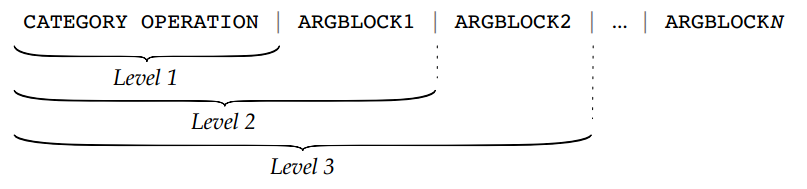
\includegraphics[width=0.7\columnwidth]{Figures/mist.png}
	\caption{\gls{mist} representation as seen in \cite{rieck:dynamic}}
	\label{fig:mist}
\end{figure}

An example of a MIST instruction could be as following:

\begin{center}\texttt{03 05 | 0100000001 | 00006ce5 | 000066fc}\end{center}

This instruction contains four levels.
The first level contains the category and operation, while the remaining levels each contain an argument block.
By variating the level, different granularities can be achieved.

The authors create a vector space for each report that represents the behavior of the sample.
The vector is conceived by creating \textit{Q-grams}.
These are the result of applying a sliding window of size $q$ to the MIST report and constructing a binary vector where every position is whether the report contains the sequence of size $q$ or not.
The size of the vector varies with the number of possible instructions and the size $q$ of the window.

The authors implement their own clustering and classification algorithms for the task at hand.
The evaluation data consists on two sets, a reference set of 3,133 malware reports with 24 different malware families, to be used to evaluate and calibrate the framework, and an application set of 33,698 unknown malware reports taken over a course of seven days.

On the reference set authors apply F-measure for evaluation, which uses precision and recall as parameters, the maximization of F-measure reflects high precision and recall.
The results yield an F-measure over 0.936, which surpasses previous research for both clustering and classification.

On the application dataset authors apply their methodology and achieve 434 clusters (\ie\ malware families).
To the ten largest clusters authors take the most frequent anti-virus label for each cluster using Kaspersky anti-virus.
They note that one anti-virus label is prevalent for each of the ten clusters, assuming that their framework successfully discovers and classifies unknown malware families.

By applying their framework to two different sets, where one was created from real-world samples, the authors show how their framework is applicable to a real-world scenario.

\subsection{Pitfalls of Using Classical Validation Methodologies}

Miller et al.~\cite{miller:rev_int} provide a system which relates to \cite{nissim:al_pdf}, as it applies expert reviewers as a limited labeling resource.
Their work uses both static and dynamic features to detect malware and uses manual label together with \gls{ml} to improve the overall result.
The authors evaluate their design on an enormous dataset of 1.1 million binaries spanning 2.5 years, taken from submissions made at VirusTotal, a service similar to Malwr.
Alongside the enormous dataset, the authors also make sure that training data predates evaluation data, contributing to an evaluation with high realism.

With regards to the design of the system, it consists of a detection and a training pipeline.
The detection pipeline takes a binary, extracts the features and applies the current model to classify the binary as malicious or benign.
The training pipeline takes binaries labeled by the manual reviewer, VirusTotal and from the current model, extracts the features and trains the new model.

The system uses multiple static and dynamic features from binaries, including: binary metadata, digital signing, static imports, dynamic imports, file operations, mutex operations, network operations, processes and Windows \gls{api} calls.
The authors chose to use \acrfull{lr} as the classifier, basing their choice on the fact that it predicts a real-valued quantity, which enables the use of a threshold and therefore allows the creation of a tradeoff between true and false positive rates, by adjusting the threshold.
\gls{lr} also assigns a weight to each feature, which allows to comprehend which features are more discriminating.

On evaluation, authors show that when ignoring temporal consistency, results inflate up to 20\% at a 0.5\% false positive rate.
When considering temporal consistency, results range from 65\% to 75\% true positive rate with a false positive rate range from 0.1\% to 1\%.

Another remark made in this article is that vendors prefer false negatives over false positives (\ie\ wrongly classifying malware as goodware over wrongly classifying goodware as malware).
When looking at duplicated samples, 29.6\% of those samples increased in the number of detections as malware and only 0.25\% decreased the number of detections.

\medskip

On the topic of methodologies that resemble real-world conditions, Srndi\'c et al.~\cite{vsrndic2013detection} train and validate their malicious PDF detector under laboratory and real-world conditions.
Laboratory conditions consist on applying regular cross-validation, whereas real-world conditions validate a newer dataset with a model created from outdated data (\ie\ older then the validation), and also validate the model when the validation set spans one week and the training is gathered in the previous 4 weeks.
They show that laboratory conditions inflate the results, when compared to real-world conditions.

Our work enhances these methodologies by analyzing the performance variation when the distance between the training and validation set increases and decreases, as well as analysis on how reducing the size of the training without compromising the results.

\medskip

Kolter et al.~\cite{kolter:learning} learn to detect malicious executables in a dataset with under 4,000 samples, obtained from reliable sources, and evaluate their model under standard cross-validation and by gathering newer malware samples to validate for new and unseen samples.
They show how the model provides optimal results under cross-validation, but for the unseen samples lower scores are obtained.
Our work considers these results to compare how reliability affects performance.

Deo, A. et al.~\cite{deo2016prescience} focus over the problem of \gls{ml} models becoming antiquated over time, given how malware evolves.
This problem is seen as concept drift, where the performance of a model over time diminishes, as the statistical properties of malware (\ie\ features) change over time.
They study how probabilistic predictors can help minimize the aforementioned problem, by indicating when retraining of a given model is necessary. 

Jordaney, R. et al.~\cite{jordaney2017transcend} also study the problem of concept drift in malware classification models, focusing on providing metrics, based on statistical comparison of samples, to detect when should a model be retrained. 

Both \cite{deo2016prescience} and \cite{jordaney2017transcend} are on the subject of our work, regarding the problem of concept drift, but differ on the study-case.
In our work we acknowledge the concept but focus on its relative effects and how one can balance the size of needed training data \textit{vs.}\ validation data, when maintaining a temporal consistent dataset.
Whereas their work provide indicators for when should a model be retrained when the problem of concept drift becomes significant.

\medskip

Perdisci et al.~\cite{perdisci:behavior} use an unsupervised learning approach to cluster malware using malicious network traces.
Although their work does not directly relate to the current work, it also deals with the malware naming problem.
To validate the obtained clusters, the cohesion and separation among clusters is measured in terms of the labels given by anti-virus vendors.

To derive the cohesion and separation, a graph for each cluster is constructed.
Each node is a malware label given by some vendor and an edge connects two nodes if the labels appear together in any malware sample.
Weights are assigned as $1 - \dfrac{m}{n}$, where $m$ is the number of times the different labels appear together and $n$ is the number of samples in the cluster.
From the graphs authors can then measure the cohesion and separation of clusters.

The authors use the aforementioned method to evaluate their results, but the approach can be useful to label and balance malware datasets that contain various anti-virus labels.

\medskip

Regarding the malware naming problem, Sebastián, M. et al.~\cite{sebastian2016avclass} develop \textit{AVClass}, a tool that given a set of antivirus vendors, outputs the most likely family name.
They test their tool under 10 datasets, totaling 8.9 million samples, with results showing an F1 measure up to 93.9\% on labeled datasets.
The tool takes as input the labels as seen in VirusTotal, tokenizes the labels, replaces known aliases and general names (\eg\ win32, trojan, generic), ending with possible family names. These remaining names are counted and the most frequent one is given as family name, Figure \ref{fig:avclass} exemplifies the stated process.

\begin{figure}[!htb]
	\centering
	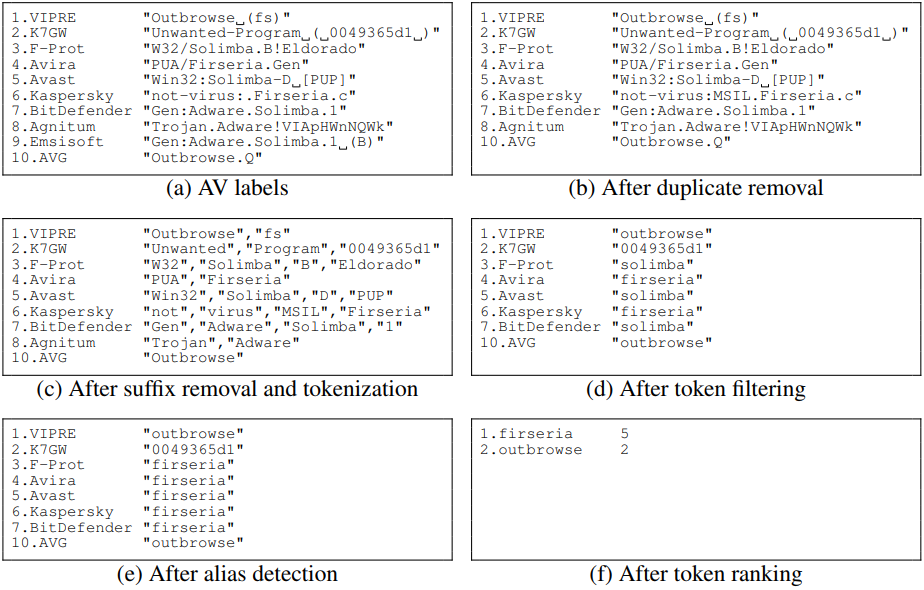
\includegraphics[width=\columnwidth]{Figures/avclass.png}
	\caption{AVClass running example.}
	\label{fig:avclass}
\end{figure}

Our work takes advantage of this tool, not to label malware families, but with minimal modifications, to label more general malware classes (\eg\ trojan, virus).

\medskip

Overall the presented research provides useful insight for the current work. Decisions like the handling of the dataset, how and which features are to be extracted from samples, which and why \gls{ml} classifiers should be used and how and why the evaluation should be made.
